\chapter{Forforstærker}

Forforstærkeren har til opgave at forstærke mikrofonens udgangssignal til et liniesignals niveau. Et liniesignal har en amplitude fra 200 mV til 2 V og mikrofonens udgangssignal ligger, ifølge standarderne, mellem 0.8 mV og 200 mV \fixme{Den er jeg ikke helt sikker på}. 
Kravene fra kravspecifikationen som har indflydelse for designet af forforstærkerne er vist i tabel \ref{tab:krav_forforstaerker}.

\begin{table}[h]
\centering
\begin{tabular}{l|r|l}
\hline\hline
Område & Krav & Baggrund for krav \\
\hline\hline
Total Harmonic Distortion & \color{red}{<1 \%} & Ref til THD afsnit \\
Indgange & Linie og mikrofon & Se afsnit \ref{standarder} \\
Indgangsvælger & 3 trin & Se afsnit \ref{krav_indgangsvaelger} \\
Udgangssignaltype & Mono & Se afsnit \ref{krav_udgangssignaltype} \\
\textbf{Frontpanel:} & & \\
Indgangsvælger & Ja & Se afsnit \ref{krav_indgangsvaelger} \\
\textbf{Fjernbetjening:} & & \\
Indgangsvælger & Ja &  Se afsnit \ref{krav_fjernbetjening}\\
\hline\hline
\end{tabular}
\caption{Krav fra kravspecifikationen som har indflydelse på forforstærkeren}
\label{tab:krav_forforstaerker}
\end{table}



\section{Design}
Forforstærkeren skal indeholde to blokke: En differensforstærker og en Common emitter (CE) forstærker med uafkoblet emittermodstand. Grunden til at forforstærkeren skal indeholde en differensforstærker er for at udnytte mikrofonens balancerede output, for derved at minimere indstrålingsstøj. CE forstærkerens opgave er, efter differensforstærkeren, at forstærke signalet således at det er på niveau med et linjesignal. På figur \ref{blok_forforstaerker} ses et blokdiagram over forforstærkerens opbygning. 

\begin{figure}[h]
\centering
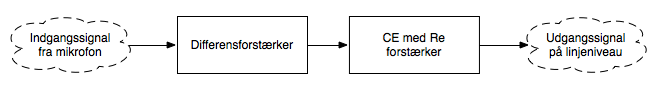
\includegraphics[scale=.6]{implementering/forforstaerker/blok_forforstaerker.png}
\caption{Blokdiagram over forforstærkerens byggeblokke samt lydsignalets vej}
\label{blok_forforstaerker}
\end{figure}

\subsection{Differensforstærker}

\subsection{CE med Re forstærker}


\section{Simulering}


\section{Accepttest}

